% !TeX spellcheck = de_DE
\section{Parallelisierung}
\label{sec:parallel}
In den vorherigen Kapiteln ist der Ablauf und die Funktionsweise von neuroevolutionären Algorithmen erläutert. Die benötigte Ausführungszeit ist von der Größe des \ac{KNN}, der Komplexität des Problems und der Populationsgröße abhängig. Für die Optimierung großer \ac{KNN} können trotz Verwendung aktueller Hardware Trainingszeiten von mehreren Stunden oder Tagen benötigt werden \cite{such2017deep}. Diese Zeit kann durch Weiterentwicklungen von einzelnen Prozessoren zunehmend verringert werden. Allerdings ist der Leistungsanstieg von neuen Prozessorgenerationen nicht ausreichend, um die benötigte Rechenzeit von solch anspruchsvollen Anwendungen massiv zu senken und skaliert somit in diesem Anwendungskontext schlecht. Zusätzlich ist die Aktualität der Prozessoren mit großem finanziellen Aufwand verbunden \cite{swann2002maximum}. Die Parallelisierung ist ein weiterer Ansatz, um die benötigte Ausführungszeit zu verringern. Hierbei wird ein großes Problem in mehrere kleine, voneinander unabhängige Teilprobleme zerlegt. Diese können dann auf verschiedenen Prozessoren gleichzeitig berechnet werden \cite{swann2002maximum}. Häufig wird in diesem Zusammenhang auch der Begriff \ac{HPC} verwendet, auf welchen im Folgenden näher eingegangen wird.

\subsection{High Performance Computing}
Das \ac{HPC} beschäftigt sich mit verschiedenen Bereichen der parallelen Programmierung. Hierzu gehören unter anderem die benötigte Software, Programmiersprachen, Tools sowie die Hardware. Zusammenfassend ist festzustellen, dass sich der Bereich des \ac{HPC} mit der Forschung, Entwicklung und dem Betreiben von \acp{SC} beschäftigt. Dies sind Cluster, welche aus mehreren Millionen \acp{CPU} bestehen und zum Lösen von verschiedenen parallelisierbaren Problemen aus Forschung und Industrie verwendet werden können \cite{nielsen2016introduction}. Eine Liste mit den $500$ leistungsfähigsten \acp{SC} ist in Quelle \cite{top500} zu finden. Stand Juni 2020 ist der leistungsfähigste \ac{SC} in Japan, welcher über sieben Millionen Prozessoren besitzt und eine Leistung von über $500.000$ TFlops bietet. Aufgrund hoher Kosten, die unter anderem durch den Stromverbrauch entstehen, sind \ac{SC} für viele Probleme nicht rentabel. Dennoch gibt es einige Anwendungsszenarien für solche Systeme.
\\\\
Häufig werden \ac{SC} für verschiedene Simulationen eingesetzt, deren Durchführung in realer Umgebung zu teuer oder zu gefährlich ist und für die als Beispiel ein Flugzeugabsturz oder die Auswirkungen nuklearer Waffen zu benennen sind. Ein weiterer Grund für den Einsatz von SC liegt vor, wenn die Berechnung oder Simulation auf einem gewöhnlichen Gerät zu viel Zeit benötigt oder wenn das Ergebnis nur eine gewisse Zeit gültig bzw. verwendbar ist. Ein Problem dieser Kategorie ist beispielsweise die Wettervorhersage. Ist es nicht möglich, das Ergebnis rechtzeitig zu erhalten, ist die Vorhersage obsolet. Nicht zuletzt ist auch die Analyse von großen Datenmengen, die nicht auf einem einzelnen Gerät effizient durchführbar ist, eine Einsatzmöglichkeit von \ac{SC} \cite{nielsen2016introduction}.

\subsubsection{Architektur}
\label{subsubsec:hpc_architecture}
Die Architekturen von \ac{HPC} Systemen sind einer von zwei Kategorien zuzuordnen, welche als \emph{shared memory} und \emph{distributed memory} bezeichnet werden. Bei der \emph{shared memory} Architektur verwenden typischerweise alle Prozessoren des Systems denselben Programmspeicher, der auch als \ac{RAM} bezeichnet wird. Die Kommunikation zwischen den Prozessoren ist in vielen Fällen durch \ac{OpenMP} realisiert \cite{nielsen2016introduction}. Diese Art der Parallelisierung kann auch auf Computersystemen angewendet werden, die für den Massenmarkt produziert wurden. Moderne \acp{CPU} besitzen auf demselben Chip mehrere physische Prozessoren, welche zur Parallelisierung von verschiedenen Anwendungen verwendet werden können und häufig die Ausführungszeit bedeutend reduzieren. 
\\\\
Die Alternative hierzu ist die \emph{distributed memory} Architektur, bei der jeder Prozessor seinen eigenen \ac{RAM} besitzt. Im Gegensatz zu \emph{shared memory} Architekturen können die Prozessoren dieser Art nicht auf Speicherbereiche von anderen Prozessoren zugreifen. Um eine Kommunikation zwischen den einzelnen Prozessoren zu ermöglichen, müssen sie explizite Nachrichten untereinander austauschen. Die Ausführungsgeschwindigkeit bzw. die Effizienz der parallelisierten Anwendung ist nicht nur von den einzelnen Prozessoren abhängig, sondern auch von der Latenz, Bandbreite und Netztopologie. Die Latenz beschreibt hierbei die Zeit, welche benötigt wird, eine Kommunikation zu initiieren, die Bandbreite die Übertragungsgeschwindigkeit der Daten. Neben diesen beiden Architekturen gibt es noch weitere Formen, welche auch \acp{GPU} nutzen können \cite{nielsen2016introduction}. Auf diese wird nicht weiter eingegangen, da in dieser Arbeit ein System mit einer \emph{distributed memory} Architektur verwendet wird.

\subsubsection{Beowulf-Cluster}
\label{subsubsec:beowulf_cluster}
Durch enorme Kosten, die in der Anschaffung spezialisierter Hardware \cite{brown2004engineering} sowie im Betrieb eines \ac{SC} \cite{nielsen2016introduction} entstehen, ist ein solches System für die meisten Unternehmen, Universitäten oder Hochschulen finanziell nicht tragbar. Dennoch kann der Einsatz kleinerer Cluster zum Beispiel in der Lehre oder für weniger rechenaufwendige Probleme, welche trotzdem von einer Parallelisierung profitieren, sinnvoll sein. 
\\\\
In einem solchen Szenario sind sogenannte Beowulf-Cluster eine mögliche Lösung. Diese haben zwar bedeutend weniger Leistung, sind dafür aber in der Anschaffung sowie im Betrieb um ein Vielfaches günstiger und eignen sich somit auch für Privatpersonen \cite{adams2008microwulf}. Diese Cluster zeichnen sich in Abgrenzung zu professionellen \ac{SC} unter anderem dadurch aus, dass die Hardware für den eigentlichen Beowulf-Cluster aus serienmäßig für den Massenmarkt produzierten Geräten zusammengesetzt werden kann. Gleiches gilt auch insofern für die Netzwerkinfrastruktur, dass ein Cluster aus mehreren Desktopgeräten bestehen kann, welche über ein Ethernet-Netzwerk miteinander verbunden sind. Weitere Anforderungen sind, dass alle Geräte des Clusters nur \emph{Open-Source}-Software verwenden, das Netzwerk exklusiv für die Kommunikation des Beowulf-Clusters reserviert ist und das Aufgabengebiet im Bereich des \ac{HPC} liegt \cite{brown2004engineering}. Diese Anforderungen müssen für einen klassischen Beowulf-Cluster erfüllt sein, dennoch gibt es verschiedene abgewandelte Varianten für andere Einsatzszenarien.
\\\\
Typischerweise basiert das Betriebssystem der einzelnen als \emph{Nodes} bezeichneten Geräte auf Linux, worin sich eine Eigenschaft verdeutlicht, welche auf die meisten Beowulf-Cluster zutrifft, aber keine Voraussetzung ist. Häufig wird ein \emph{Node} als \emph{Master} ausgewählt, der als Schnittstelle zwischen dem eigentlichen Cluster und der externen Umgebung dient, die restlichen \emph{Nodes} werden als \emph{Slaves} bezeichnet. So kommt es häufig vor, dass der \emph{Master} über eine angeschlossene Tastatur und einen Bildschirm verfügt, welche eine Interaktion mit dem Cluster ermöglichen. Zusätzlich hat dieser häufig als einziges Gerät neben der Verbindung zu den \emph{Slaves} auch eine externe Netzwerkanbindung. Dies wird benötigt, da der \emph{Master} in der Regel viele organisatorische Aufgaben übernimmt. Beispiel hierfür kann das Bereitstellen und die Synchronisation von Dateien im Netzwerk sein \cite{brown2004engineering}.
\\\\
Aufgrund der vergleichsweise niedrigen Kosten sowie der einfachen Anschaffung und Inbetriebnahme bieten sich solche Cluster für viele verschiedene Projekte an. Auch in dieser Arbeit wird ein Beowulf-Cluster verwendet, auf dessen Installation und Konfiguration in Kapitel \ref{sec:test_env_parallel} eingegangen wird.

\subsubsection{MPI und MapReduce}
\label{subsubsec:mpi_and_mapreduce}
Für eine erfolgreiche Parallelisierung in einem \emph{distributed memory} System, wie zum Beispiel in einem Beowulf-Cluster, müssen sich die einzelnen Prozessoren untereinander synchronisieren sowie Nachrichten austauschen können. Hierfür gibt es verschiedene Bibliotheken, welche einen Großteil dieser Funktionen bereitstellen. Beispiele hierfür sind \ac{MPI} und \emph{MapReduce}. Diese unterscheiden sich in ihrer Funktionalität und der Umgebung, in welcher sie eingesetzt werden \cite{nielsen2016introduction}.
\\\\
Die Verwendung von \ac{MPI} in dieser Arbeit, welches in Kapitel \ref{subsec:mpi} genauer erläutert wird, ist unter anderem in seinem Vorteil begründet, dass eine Vielzahl verschiedener Kommunikations- und Synchronisationsoperatoren implementiert sind, welche flexibel an viele Anforderungen angepasst werden können. Allerdings besteht keine Fehlertoleranz gegenüber Hardware- und Netzwerkfehlern. Treten diese auf, bricht die Ausführung der gesamten Anwendung ab und nicht gespeicherte Zwischenergebnisse gehen verloren. Bezüglich diesen Aspekts bietet die Alternative \emph{MapReduce} einen Vorteil, da diese Fehler automatisch verarbeiten kann. Nachteil gegenüber \ac{MPI} ist, dass nicht so viele verschiedene, flexible Funktionen der Parallelisierung geboten werden \cite{nielsen2016introduction}.

\subsection{MPI}
\label{subsec:mpi}
Wie in den vorherigen Kapiteln erläutert, müssen in einem parallelen System die Prozessoren miteinander kommunizieren können. Vor allem bei Systemen mit einer \emph{distributed memory} Architektur wird häufig \ac{MPI} verwendet, welches ein anerkannter Standard im Bereich des \ac{HPC} ist. Zusätzlich kann \ac{MPI} auch auf \emph{shared memory} Architekturen angewendet werden. Die erste Version des Standards wurde bereits 1991 entwickelt \cite{nielsen2016introduction}. Im Jahr 2008 wurde die derzeit aktuelle Version 3 veröffentlicht. Bevor die verschiedenen Funktionen von \ac{MPI} vorgestellt werden, wird zunächst auf einige Besonderheiten eingegangen. Der Standard \ac{MPI} ist keine konkrete Implementierung, sondern ein \ac{API}, welches nur die grundsätzliche Funktionsweise sowie einige Basisoperationen definiert \cite{nielsen2016introduction}. Einer der sich ergebenden Vorteile ist darin zu verdeutlichen, dass die Implementierung des Standards nicht an eine einzelne Programmiersprache geknüpft ist \cite{nielsen2016introduction}. Dies gibt Herstellern die Möglichkeit, ihre eigene Implementierung in jeder gewünschten Sprache umzusetzen. Hieraus sind viele kommerzielle Produkte entstanden, aber mit \emph{MPICH} und \emph{Open MPI} auch zwei bekannte \emph{Open-Source}-Lösungen. Diese können als Bibliotheken in andere Projekte eingebunden werden und vereinfachen die Entwicklung einer parallelen Anwendung enorm, da verschiedene \emph{low-level} Funktionen, wie beispielsweise die Netzwerkkommunikation, bereits implementiert sind. Des Weiteren ermöglicht der \ac{MPI} Standard eine hohe Portabilität, da Implementierungen mit wenig Aufwand ausgetauscht werden können und auf einer Vielzahl von Systemen lauffähig sind \cite{dalcin2008mpi}.
\\\\
Die Funktionen von \ac{MPI} können heutzutage in verschiedenen Sprachen, wie zum Beispiel Java, C, C++, Python und Fortran verwendet werden \cite{nielsen2016introduction}. Im Folgenden wird auf die wichtigsten Grundfunktionen von \ac{MPI} eingegangen. Der Beispielcode ist in der Sprache Python und der Bibliothek \emph{mpi4py} aus Quelle \cite{dalcin2008mpi} implementiert. Diese werden auch im weiteren Verlauf dieser Arbeit verwendet.
\subsubsection{Prozessorgruppen}
Bevor die verschiedenen Kommunikations- und Synchronisationsmöglichkeiten vorgestellt werden, muss der grundlegende Ablauf eines auf \ac{MPI} basierenden Programms betrachtet werden. Beim Starten eines solchen Programms wird auf jedem der beteiligten Prozesse, welche in einer Konfigurationsdatei spezifiziert sind, eine Kopie des Programms ausgeführt. Eine grundlegende Voraussetzung ist, dass das Programm auf allen beteiligten \emph{Nodes} vorliegt. 
\\\\
Die sogenannten \emph{Communicators}, im Programmcode auch häufig mit \emph{COMM} abgekürzt, sind Gruppen von verschiedenen Prozessen, welche miteinander kommunizieren können. Beim initialen Starten des Programms wird nur eine Prozessgruppe erstellt, welche alle beteiligten Prozesse enthält und als \emph{MPI\_COMM\_WORD} bezeichnet wird. Jeder Prozess in einem \emph{Communicator} wird  durch einen Rang zwischen $0$ und $P-1$ identifiziert, wobei $P$ die Anzahl an Prozessen ist \cite{nielsen2016introduction}. Der Rang sowie die Anzahl der Prozesse können im Programmcode angefragt und als Grundlage für verschiedene Entscheidungen genutzt werden. Ein Beispiel hierfür ist in Abbildung \ref{fig:example_process_group} dargestellt. Der gegebene Programmabschnitt wurde mit zwei Prozessoren ausgeführt. An der Ausgabe ist erkennbar, dass die Anweisung \emph{print()} von jedem Prozess einmal aufgerufen wird und sich lediglich die Variable \emph{rank} unterscheidet. 
\begin{figure}
	
	\begin{python}
		from mpi4py import MPI
		
		comm = MPI.COMM_WORLD
		rank = comm.Get_rank()
		size = comm.Get_size()
		
		print("Hello world, Rank:", rank, ", Size:", size)
		
		>>> Hello world, Rank: 1, Size: 2
		>>> Hello world, Rank: 0, Size: 2
	\end{python}
	\caption{\emph{HelloWord} MPI Programm in Python}
	\label{fig:example_process_group}
\end{figure}



% MPI Communicaor, splittet Processe in Auf, 
% Aktuell Version 3
% Ursprünglich 80 Personen und 30 Organisationen, Attraktiv because Protability and Scalability, Distributed and Shared Memory Multiprocesses
% Standard defacto von HPC
% Blocking Non Blocking
\subsubsection{Point-to-Point Kommunikation}
\label{subsubsec:point_to_point_communication}
Typischerweise wird \ac{MPI} unter anderem zum Austauschen von Nachrichten verwendet. Bei der in diesem Abschnitt vorgestellten, sogenannten \emph{Point-to-Point} Kommunikation sendet ein Prozess entweder synchron oder asynchron Daten an einen anderen \cite{nielsen2016introduction}. Abbildung \ref{fig:example_point_to_point} zeigt ein Beispiel für die synchrone Kommunikation, in der die \emph{send()} und \emph{recv()} Funktion zum Einsatz kommen. Die \emph{send()} Funktion versendet Daten an einen anderen Prozess. Als Parameter müssen die zu sendenden Daten und das Ziel übergeben werden. Dieses wird durch den entsprechenden Rang identifiziert. Optional kann der Funktion noch ein \emph{tag} übergeben werden, welches zusätzliche Informationen zu den Daten enthält. Beispielsweise kann dieses verwendet werden, um dem Zielprozess zu signalisieren, wie die Daten verarbeitet werden sollen. Die \emph{recv()} Funktion wird zum Empfangen der Daten verwendet. Diese kann prinzipiell ohne Parameter aufgerufen werden, sodass jede Nachricht von jedem Prozess akzeptiert wird. Sollen spezielle Nachrichten mit einem gewissen \emph{tag} oder von einem spezifischen Prozess empfangen werden, ist dies durch Übergeben von weiteren Parametern möglich. Dies kann wichtig sein, wenn Nachrichten beispielsweise in einer gewissen Reihenfolge empfangen werden müssen. 
\begin{figure}
	\begin{python}
		from mpi4py import MPI
		
		comm = MPI.COMM_WORLD
		rank = comm.Get_rank()
		size = comm.Get_size()
		
		if rank == 0:
			data_to_send = 42
			comm.send(data_to_send, dest=1)
			print("Data sent: ", str(data_to_send))
		elif rank == 1:
			data_recv = comm.recv()
			print("Data received: " + str(data_recv))
			
		>>> Data sent:  42
		>>> Data received: 42
	\end{python}
	\caption{\emph{Point-to-Point} Kommunikation mit \ac{MPI} in Python}
	\label{fig:example_point_to_point}
\end{figure}
\\ \noindent
Eines der Probleme, das potenziell durch die synchrone Kommunikation verursacht wird, betrifft die Effizienz, da sowohl die \emph{send()} als auch \emph{recv()} Funktion die weitere Ausführung des Programmcodes blockieren, bis die Übertragung erfolgreich abgeschlossen ist. Sollte einer der beiden Prozesse ausgelastet sein, wird der andere auf ihn warten und in dieser Zeit keine Berechnungen durchführen \cite{nielsen2016introduction}. Kommen diese Wartezeiten häufig und lange vor, kann dies die Performanz des Systems stark beeinträchtigen. Ein weiteres Problem besteht darin, dass Fehler im Programmcode zu \emph{Deadlocks} führen können. Eine solche Situation kann entstehen, wenn zwei Prozesse eine Nachricht vom jeweils anderen erwarten und daher nicht mit der Programmausführung fortfahren \cite{nielsen2016introduction}. Da kein Prozess eine Nachricht schicken wird, muss das Programm in einem solchen Fall extern manuell beendet werden und alle nicht gespeicherten Zwischenergebnisse gehen verloren. Um diese Probleme zu umgehen, kann die asynchrone Variante der \emph{Point-to-Point} Kommunikation verwendet werden, welche mit den Funktionen \emph{isend()} und \emph{irecv()} implementiert ist. Möchte ein Prozess Daten senden bzw. empfangen und ist der Kommunikationspartner noch nicht bereit, wird mit der Ausführung des Programmcodes fortgefahren. Wenn der Kommunikationspartner letztendlich für die Übertragung bereit ist, wird diese automatisch gestartet \cite{nielsen2016introduction}. 

\subsubsection{Gruppenkommunikation}
Der \ac{MPI} Standard definiert nicht nur die \emph{Point-to-Point} Kommunikation, sondern auch verschiedene Formen der Gruppenkommunikation. Diese können in einigen Fällen bedeutend effizienter sein, als Nachrichten mit allen Prozessen einzeln auszutauschen. Einige der wichtigsten Operationen sind die \emph{Broadcast}, \emph{Scatter}, \emph{Gather} und \emph{Reduce} Funktion, welche beispielhaft in Abbildung \ref{fig:mpi_group_communication} dargestellt sind \cite{dongarra1995introduction}.
\begin{figure}[!h]
	\centering
	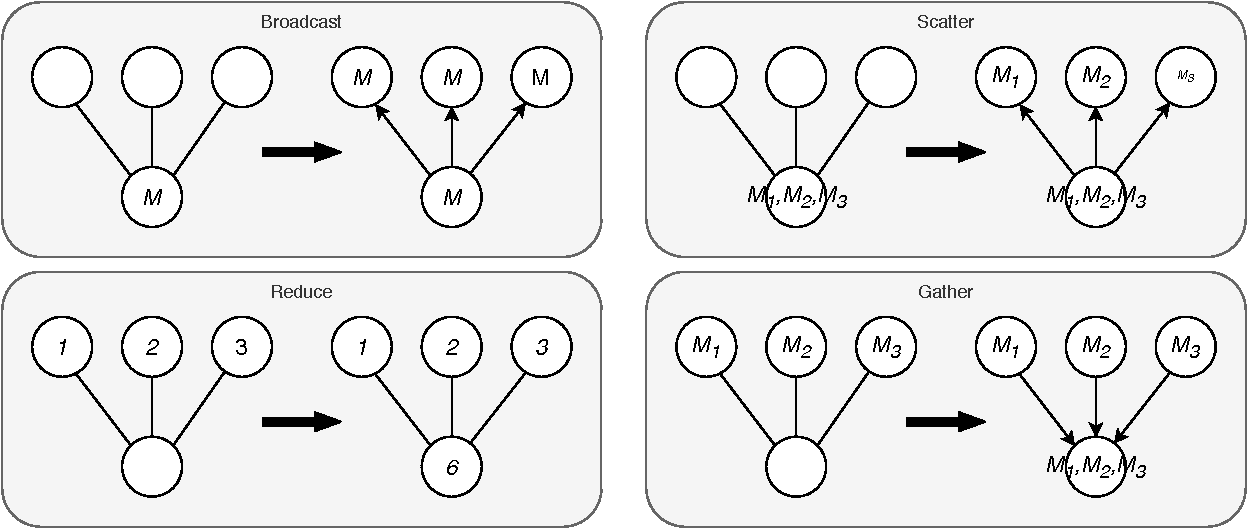
\includegraphics[width=1\textwidth]{./img/mpi_group_communication.pdf} 
	\caption{Schematische Darstellung der \emph{Broadcast}, \emph{Scatter}, \emph{Gather} und \emph{Reduce} Funktion in MPI}
	\label{fig:mpi_group_communication}
\end{figure}
\\ \noindent
Mit der \emph{Broadcast} Funktion kann ein Prozess eine Nachricht $M$ an alle anderen beteiligten Prozesse senden \cite{dongarra1995introduction}. Diese einfache Operation wird in vielen Fällen benötigt, wenn beispielsweise der \emph{Master} Prozess in einem Cluster Daten an alle \emph{Slaves} senden muss. Mit der \emph{Scatter} Funktion kann ein Prozess die Elemente einer Liste bzw. eines Arrays gleichmäßig an die anderen Prozesse verteilen, sodass jeder Empfänger nur einen Teil der Daten erhält \cite{nielsen2016introduction}. Diese Operation kann eingesetzt werden, wenn für jedes Element der Liste eine vom Rest unabhängige Berechnung durchgeführt werden muss. Zwar wäre es in einem solchen Szenario auch möglich, die \emph{Broadcast} Funktion zu verwenden und dann basierend auf dem Rang die Berechnung durchzuführen, aber bei der \emph{Scatter} Funktion werden insgesamt weniger Daten übertragen und somit eine geringere Bandbreite benötigt. Das Pendant zur \emph{Scatter} Funktion ist die \emph{Gather} Funktion. Hierbei erhält ein Prozess von allen anderen eine Nachricht $M_i$ und aggregiert diese in einer Liste oder einem Array \cite{nielsen2016introduction}. Die \emph{Scatter} und \emph{Gather} Funktionen werden häufig zusammen verwendet. Mit der \emph{Scatter} Funktion können die Daten an die verschiedenen Prozesse verteilt werden, diese berechnen ihre Ergebnisse, welche zuletzt mit der \emph{Gather} Funktion wieder gesammelt werden. Die letzte hier vorgestellte Funktion wird \emph{Reduce} genannt. Mit dieser können verschiedene globale Berechnungen mit einem binären kommutativen Operator durchgeführt werden \cite{nielsen2016introduction}. Eine Rechenoperation ist kommutativ, wenn für alle $a$ und $b$ einer Menge $M$  die Gleichung $a*b=b*a$ gilt \cite{walz2011brueckenkurs}. In Abbildung \ref{fig:mpi_group_communication} wird die Summe berechnet, aber \ac{MPI} bietet darüber hinaus andere Standardoperatoren, wie die Berechnung des Produkts, Minimums oder Maximums \cite{nielsen2016introduction}. 
\\\\
\ac{MPI} bietet noch weitere Arten der Gruppenkommunikation, auf welche an dieser Stelle nicht ausführlich eingegangen wird. Die \emph{AllGather} Funktion kombiniert die \emph{Gather} Funktion mit einem anschließenden \emph{Broadcast} des Ergebnisses. Bei der \emph{AllToAll} Funktion besitzt jeder Prozess eine Liste und sendet jeweils ein Element an jeden anderen Prozess \cite{dongarra1995introduction}. Eine spezielle Art der Gruppenkommunikation sind die sogenannten Synchronisationsbarrieren, an denen die Ausführung der einzelnen Prozesse angehalten wird, bis alle Teilnehmer diese erreicht haben \cite{nielsen2016introduction}. Abschließend sind zwei Anmerkungen zu nennen, welche für die verschiedenen Arten der Gruppenkommunikation wichtig sein können. Erstens ist jede dieser Operationen nur als synchrone Funktion verfügbar. Die zweite Anmerkung betrifft die Synchronisationsbarrieren. Bei vielen Implementierungen haben Funktionen wie der \emph{Broadcast} einen Synchronisationsseiteneffekt. Dies ist durch den \emph{MPI} Standard möglich, jedoch keine Voraussetzung und kann somit die Portierung von Projekten beeinflussen, die von diesen Seiteneffekten abhängig sind \cite{dongarra1995introduction}.

\subsection{Performance}
\label{subsec:basics_performance}
% Eventuell load balancing, wichtig
Das Erstellen eines gut parallelisierten Algorithmus ist häufig bedeutend schwieriger als das Erstellen desselben in einer sequenziellen Variante. Der Grund hierfür ist, dass zwar jeder parallele Algorithmus sequenziell ausführbar ist, indem die unabhängigen Teilaufgaben nacheinander abgearbeitet werden, dies aber umgekehrt nicht möglich ist. Um gute Ergebnisse zu erzielen, muss der parallelisierte Algorithmus häufig neu erstellt oder umstrukturiert werden. \cite{nielsen2016introduction}. Dieses Kapitel stellt Methoden vor, mit welchen die tatsächliche und maximal zu erwartende Performance eines parallelen Algorithmus berechnet werden kann. 
\\\\
Bevor auf die genauen Berechnungen eingegangen wird, sei angenommen, dass die serielle Ausführung eines Algorithmus $t_{seq}$ lange dauert und dass $t_q$ die Zeit angibt, welche derselbe parallele Algorithmus mit $P$ Prozessoren benötigt. Der sogenannte \emph{SpeedUp} gibt an, um welchen Faktor die parallele Ausführung eines Programms schneller ist. Berechnet wird dies mit $SpeedUp(P)=\frac{t_{seq}}{t_P}$ \cite{nielsen2016introduction}. Der \emph{SpeedUp} gibt nicht an, wie gut oder schlecht die tatsächliche Parallelisierung ist. Hierfür wird die Effizienz $e$ benötigt, welche mit $e=\frac{SpeedUp(P)}{P}$ berechnet wird. An dieser kann abgelesen werden, wie gut die parallele Ausführung tatsächlich ist. Der berechnete Wert liegt meistens zwischen $0$ und $1$, wobei ein niedriger Wert ein Indiz dafür ist, dass durch die Parallelisierung und eventuelle Kommunikation viel zusätzlicher Rechenaufwand entsteht. Dementsprechend zeigt ein hoher Wert, dass wenig zusätzlicher Aufwand entsteht und die Parallelisierung effizient erfolgt. In seltenen Fällen ist es sogar möglich, dass höhere Werte als $1$ erzielt werden, was einem \emph{super-linear SpeedUp} entspricht. Dies kann vorkommen, wenn beispielsweise mehrere Prozesse denselben \emph{Cache} verwenden. Hierbei ist es möglich, dass ein Prozess Rechenzeit einsparen kann, indem er ein Ergebnis aus dem \emph{Cache} wiederverwendet, das ein anderer Prozess berechnet hat \cite{nielsen2016introduction}.
\\\\
Mit den vorgestellten Formeln lassen sich der \emph{SpeedUp} und die Effizienz berechnen, sie geben allerdings keine Auskunft darüber, was der höchst mögliche \emph{SpeedUp} bzw. die kürzeste Ausführungszeit ist. Um diese zu berechnen, gibt es zwei Theoreme, welche unter den Begriffen \emph{Amdahl's Law} und \emph{Gustafson's Law} bekannt sind \cite{nielsen2016introduction}. 
\\\\
\emph{Amdahl's Law} wurde 1967 von Gene Amdahl in seiner Arbeit in Quelle \cite{amdahll1967validity} beschrieben. Die im Folgenden vorgestellten Formeln wurden erst später hieraus abgeleitet \cite{amdahll1967validity}. Angenommen wird ein Algorithmus bestehend aus zwei Teilen, bei dem der erste Teil $\alpha_{seq}$ rein sequenziell und der zweite Teil $\alpha_{par}$ parallelisierbar ist. Weiterhin wird angenommen, dass $\alpha_{seq}+\alpha_{par}=1$ ist und dass $t_1$ die Zeit angibt, welche ein einzelner Prozess zum Ausführen eines Programmabschnittes benötigt. Die Ausführungszeit $t_P$ eines solchen parallelisierten Programms mit $P$ Prozessen kann mit $t_P=\alpha_{seq} \cdot t_1 + \alpha_{par} \cdot \frac{t_1}{P}$ berechnet werden. Um den höchsten erreichbaren \emph{SpeedUp} zu berechnen wird angenommen, dass $t_1=t_{seq}$ gilt und der erhaltene Wert $t_P$ in die bereits vorgestellte Formel für die Berechnung des \emph{SpeedUps} eingesetzt wird. Hierdurch ergibt sich die bekannte Formel von \emph{Amdahl's Law} \cite{nielsen2016introduction}: 
$$SpeedUp(P)=\frac{1}{\alpha_{seq}+\frac{\alpha_{par}}{P}}$$
Angenommen, es gäbe unendlich viele Prozessoren ($P \rightarrow \infty$), dann ist die Ausführungszeit des parallelisierbaren Programmteils vernachlässigbar gering, sodass nur der sequenzielle Anteil das Ergebnis maßgeblich beeinflusst und somit gilt \cite{nielsen2016introduction}:
$$\lim _{P \rightarrow \infty} SpeedUp(P)=\frac{1}{\alpha_{seq}}$$
Ist ein Algorithmus beispielsweise zu $95\%$ parallelisierbar und dementsprechend zu $5\%$ seriell, dann beträgt der maximale \emph{SpeedUp} für diesen $20$. \emph{Amdahl's Law} gilt unter der Annahme, dass bei steigender Prozessanzahl der Rechenaufwand der zu lösenden Aufgabe konstant bleibt, was auf viele Anwendungsszenarien zutrifft \cite{nielsen2016introduction}. Im Gegensatz hierzu steht das \emph{Gustafson's Law}, welches von John Gustafson stammt. Dieser argumentiert, dass \emph{Amdahl's Law} parallelen Systemen nicht gerecht würde, da der eigentliche Vorteil von diesen die Bearbeitung von größeren Datenmengen in derselben Zeit sei. In diesem Fall wird mit steigender Prozessanzahl ebenfalls der Rechenaufwand erhöht. Dies ermöglicht es, höhere \emph{SpeedUp} Werte zu erzielen \cite{hill2008amdahl}.



















